\chapter{Описание принципа работы подсистемы питания}
\section{Описание схемотехнического решения}
\subsection{PoE-контроллер}
\hspace{1cm} 

В измерительных приборах вопрос питания стоит особенно остро, ведь даже те помехи, которые 
не нанесли бы обычному цифровому устройству значительного вреда, могут с легкостью испортить
всю точность измерения измерительных аналоговых частей приборов. Поэтому грамотный и продуманный расчет 
подсистемы питания, основанный на опыте крупных компаний -- залог правильной и предсказуемой работы устройства.
Именно по этой причине за основу самого критического узла питания отладчика -- DC-DC преобразователя,
было взято решение компании Texas Instruments.
Подсистема питания состоит из трех частей:

\begin{enumerate}
    \item Микросхема контроллера PoE TPS2376 с обвязкой.
    \item DC-DC преобразователь LMR36520FADDA с обвязкой.
    \item LDO стабилизатор TLV1117 с обвязкой.
    \item Понижающий ШИМ-регулятор  ST1S10.
\end{enumerate}

За основу схемотехнического решения контроллера PoE взята типичная применяемая схема для
микросхемы TPS2376, которая была доработана и изображена на рисунке \ref{ris:311}.

\begin{figure}[H]
    \centering
    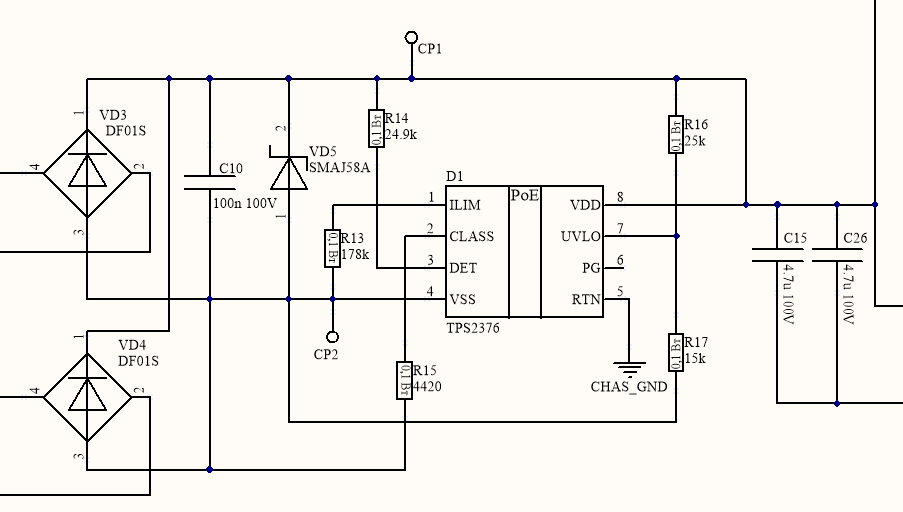
\includegraphics[scale = 0.7]{ris311.png}
    \caption{Принципиальная электрическая схема обвязки TPS2376 }
    \label{ris:311}
\end{figure}

На четвертый контакт диодного моста VD3 приходит сигнал с четвертого и пятого контактов 
Ethernet-разъема RJ45, которые отвечают за подключение отрицательного напряжения PoE.
На второй контакт диодного моста VD3 приходит сигнал с седьмого и восьмого контактов 
Ethernet-разъема RJ45, которые отвечают за подключение положительного напряжения PoE.  
На второй и четвертый контакты диодного моста VD4 приходят сигналы со средней точки согласующего
Ethernet-трансформатора с линий передачи и приема данных. Диодные мосты нужны для защиты последующей 
части устройства от различных стандартов PoE, в том числе и Passive PoE. 

Керамический конденсатор C10 является фильтрующим по питанию. Фильтрующие конденсаторы предназначены 
для фильтрации питания микросхем от высокочастотных помех и обычно их номинал равен 100 нФ.
Такие конденсаторы встречаются довольно  часто, и в дальнейшем в этой дипломной работе не будет 
описываться их назначение. Так как максимальное напряжение PoE 57 В, то рабочее напряжение 
конденсатор C10 выбрано почти с двойным запасом для повышения срока службы и надежности схемы.

Супрессор VD5 предназначен для защиты микросхемы от перенапряжения, например в случае поражения
линии статикой и рассчитан на рабочее напряжение в 58 В. 

Резистор R13 предназначен для ограничения пускового тока. Ограничение пускового тока ограничивает
протекание тока через выходные конденсаторы C15 и С26 в начальный момент их зарядки и не дает 
вызвать просадку напряжения ниже, чем задает делитель напряжения R16, R17 на выводе UVLO. 
Рекомендуемый номинал резистора -- 178 кОм.  

Обычно сопротивление резистора R14 должно быть равно 24,9 кОм. Rdet подключен к входной линии, 
когда VDD находится в диапазоне от 1,4 В до 11,3 В, и отключается,
когда напряжение на линии выходит за пределы этого диапазона, чтобы сэкономить энергию.
Этот диапазон напряжений был выбран для того, чтобы обеспечить возможность обнаружения с 
помощью двух кремниевых выпрямителей между контроллером PoE и разъемом RJ-45.

Значение резистора R15 было выбрано равным 4420 Ом исходя из 
необходимой выходной мощности по таблице \ref{ClassTPS2376} \cite{TPS2376:datasheet}.

\begin{table}[H]
    \caption{Классификация TPS2376} 
    \label{ClassTPS2376}
    \begin{center}
    \begin{tabular}{|c|c|c|c|}
    \hline
    Class & PD POWER, W  &  Rclass, Ohm   & 802.3af LIMITS, mA \\ \hline
    0 & 0,44 -- 12,95  & 4420 &0 -- 4  \\ \hline
    1 & 0,44 -- 3,84 & 953 & 9 -- 12   \\ \hline
    2 & 3,84 -- 6,49 & 549 & 17 -- 20  \\ \hline
    3 & 6,49 -- 12,95 & 357 & 26 -- 30   \\ \hline
    \end{tabular}
    \end{center}
\end{table} 

Вывод VSS подключается к минусу выходного с диодных мостов напряжения, 
а вывод VDD подключается к плюсу этого напряжения.

Вывод PG предназначен для передачи разрешающего сигнала на работу последующих микросхем,
в данной схеме нет потребности в реализации дополнительных условий или задержек включения
дальнейших элементов схемы, поэтому он не используется.

Вывод UVLO используется с внешним резисторным делителем между VDD и VSS для установки 
верхнего и нижнего порогов UVLO. TPS2376 включает выход, когда напряжение UVLO превышает верхний 
порог UVLO. Когда начинает течь ток, VDD проседает из-за сопротивления кабеля и динамического 
сопротивления входных диодов. Нижний порог UVLO должен быть ниже самого низкого напряжения, 
которого достигает вход. Коэффициент делителя должен быть выбран таким образом, 
чтобы получить примерно 1,2 В на выводе UVLO, когда VDD находится на требуемом 
напряжении включения 21 В. Поэтому R16 и R17 выбраны номиналом 25 кОм и 15 кОм соответственно.

Выходные конденсаторы С15 и С26 предназначены для фильтрации выходного напряжения, но взяты 
несколько меньше по номиналу рекомендуемых для уменьшения габаритов устройства. Их рабочее
напряжение так же взято с почти двойным запасом \cite{TPS2376:datasheet}.

Общий принцип работы этого в обеспечении стандарта IEEE 802.3af, который определяет 
процесс безопасного питания по PoE по Ethernet-кабелю и последующего отключения питания, 
если нагрузка отсоединена. Процесс проходит через три рабочих состояния: обнаружение, 
классификация и работа. Смысл процесса заключается в том, что когда нагрузка не подключена,
контроллер PoE периодически проверяет наличие подключенного устройства -- это называется 
обнаружением. Если подключается нагрузка, то контроллер может запросить информацию о том,
сколько энергии она потребует -- это этап классификации. Знание потребности в мощности нагрузки 
позволяет контроллеру PoE разумно отдавать и распределять энергию, в случае нескольких нагрузок,
а так же защищать себя от перегрузки. После этапа классификации контроллер подает питание на 
нагрузку и контролирует линию питания на предмет перегрузки. Если после этого отключить нагрузку,
контроллер снова войдет в исходное состояние обнаружения. Рисунок \ref{ris:312}  иллюстрирует 
вышеописанный паттерн поведения контроллера PoE \cite{TPS2376:datasheet}.

\begin{figure}[H]
    \centering
    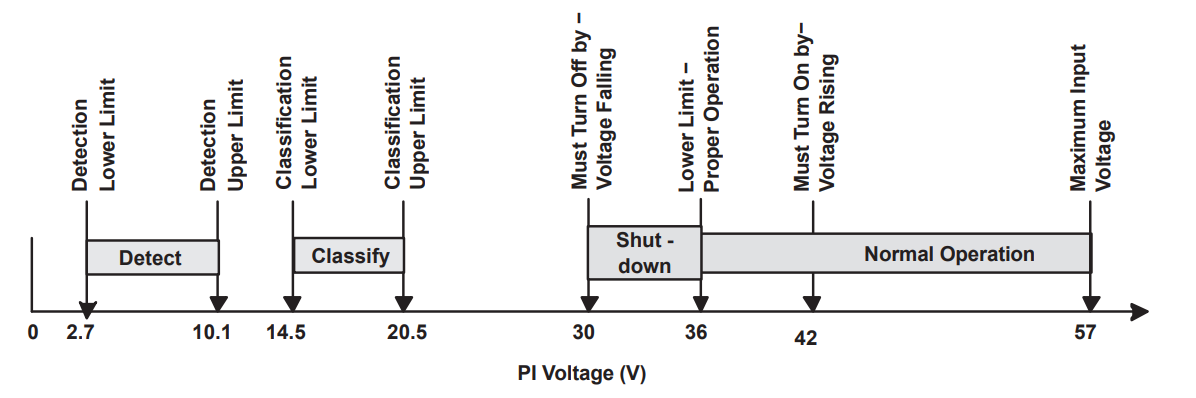
\includegraphics[scale = 0.55]{ris312.png}
    \caption{IEEE 802.3 PD Limits}
    \label{ris:312}
\end{figure}

Ожидаемые осциллограммы в основных узлах этой части схемы представлены на рисунке 
\ref{ris:313} \cite{TPS2376:datasheet}.

\begin{figure}[H]
    \centering
    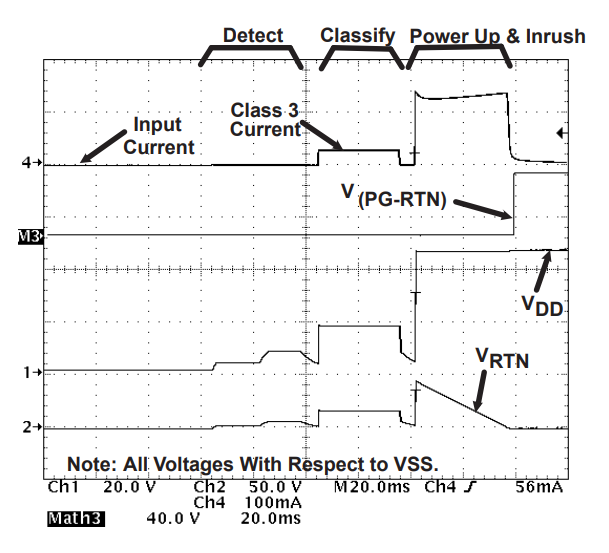
\includegraphics[scale = 0.75]{ris313.png}
    \caption{Осциллограммы TPS2376 при включении}
    \label{ris:313}
\end{figure}

\subsection{DC-DC преобразователь}
\hspace{1cm} 

В качестве изолированного Fly-Buck-преобразователя было выбрано решение на базе микросхемы LMR36520 
от компании Texas Instruments из-за наличия подробной документации по расчету каждого элемента
обвязки. 

Схемотехническое решение представлено на рисунке \ref{ris:321}.

\begin{figure}[H]
    \centering
    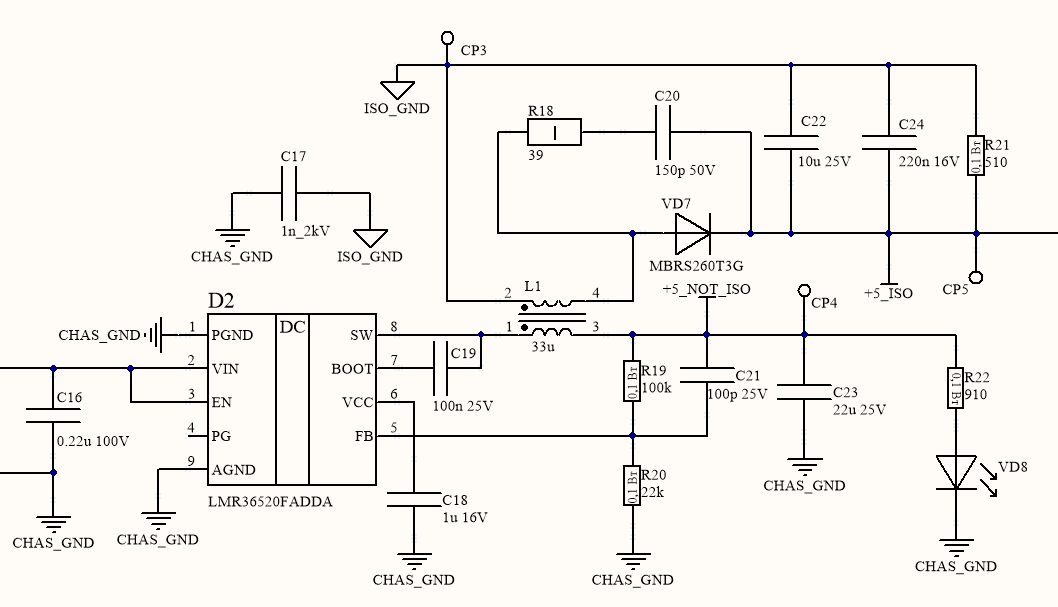
\includegraphics[scale = 0.65]{ris321.png}
    \caption{Принципиальная электрическая схема обвязки LMR36520}
    \label{ris:321}
\end{figure}

Конденсатор С16 является фильтрующим по входному питанию.На вывод VIN приходит напряжение
с выхода PoE-контроллера. Сигнал EN является разрешающим работу преобразователя. Так как
в данной схеме нет потребности в реализации дополнительных условий или задержек включения
DC-DC преобразователя, то этот вывод останется неподключенным. PGND и AGND соединены внутри 
микросхемы и подключаются к <<аналоговой>> земле. 

PG -- это выход флага состояния питания преобразователя, является выходом с открытым стоком. 
В данной схеме нет потребности в отслеживании включения преобразователя, поэтому этот вывод не 
используется. 

FB -- вход обратной связи регулятора, подключается к средней точки резистивного делителя
напряжения.

Вывод VCC является выходом внутреннего стабилизатора на 5 В, для <<собственных нужд>> преобразователя.

К выводу BOOT подключается bootstrap конденсатор, он же конденсатор запуска, номиналом 100 нФ 
\cite{LMR36520:datasheet}. 

Индуктивность L1 выполняет роль накопителя энергии в Fly-Buck преобразователях. 
Принцип работы Fly-Buck преобразователей мало отличается от Fly-Back, все основные принципы сохранены
\cite{IsoTopol},
поэтому описать работу схемы можно на примере схемы замещения для Fly-Back, 
изображенной на рисунке \ref{ris:322}.

\begin{figure}[H]
    \centering
    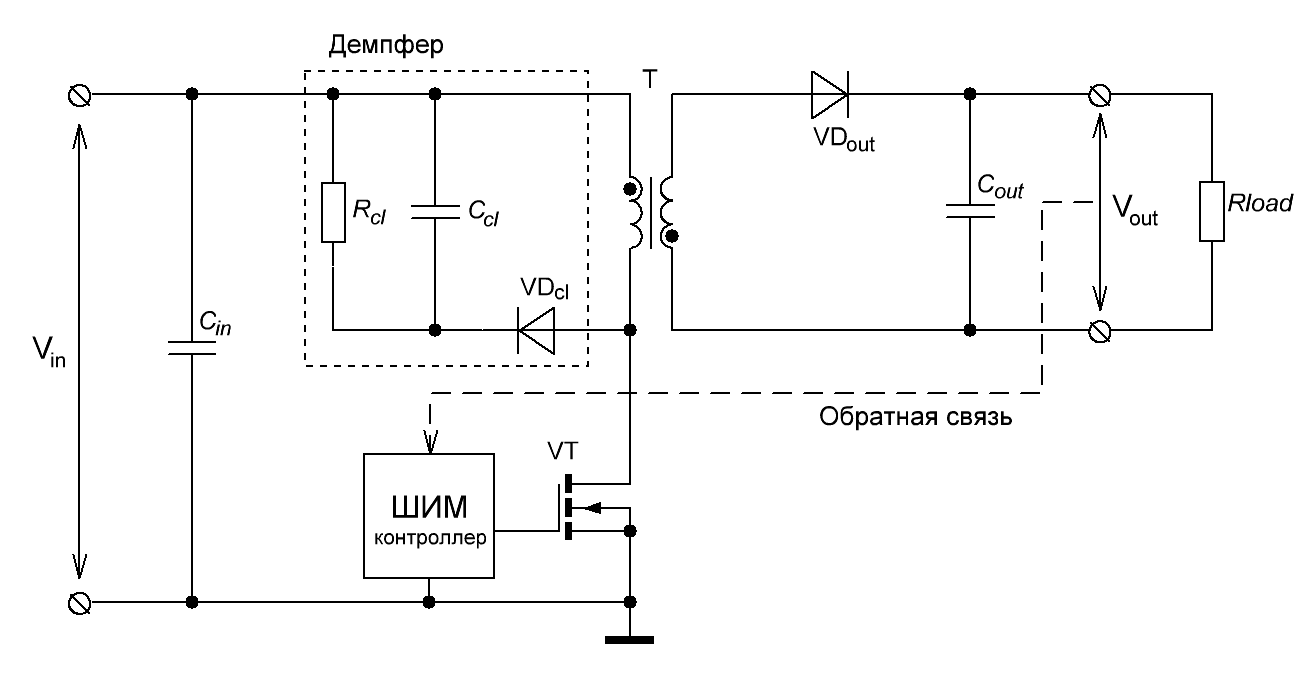
\includegraphics[scale = 0.5]{ris322.png}
    \caption{Упрощенная электрическая схема обратноходового преобразователя}
    \label{ris:322}
\end{figure}

Принцип работы обратноходового преобразователя состоит в следующем. Ключевой транзистор, 
управляемый ШИМ-контроллером, которые в рамках нашего схемотехнического решения встроены
в микросхему LMR36520, коммутирует первичную обмотку трансформатора к источнику питания.
Первичная обмотка обратноходового трансформатора фактически представляет собой дроссель, 
поэтому после коммутации ток через неё линейно растет и энергия накапливается в магнитопроводе. 
К выходному диоду приложено запирающее напряжение и ток во вторичной обмотке не протекает. 
В момент, когда транзистор закрывается, полярность на обмотках в соответствии с законом 
самоиндукции изменяется на противоположную. Диод открывается, ток начинает протекать через
вторичную обмотку трансформатора, и энергия, запасенная в магнитопроводе, переходит в нагрузку. 
И это при закрытом ключе. Далее процесс повторяется. Выходной конденсатор фильтра является 
энергетическим буфером, поддерживающем ток в нагрузке в моменты паузы.
В основе работы преобразователя лежит накопление энергии в индуктивности первичной обмотки 
на первой во времени стадии заряда и передача запасенной энергии на последующей стадии 
передачи энергии. Поскольку стадии накопления и передачи энергии разделены во времени, 
то трансформатор в обратноходовом преобразователе фактически представляет собой индуктивностью 
с двумя или более обмотками. Этот факт Мы используем для уменьшения габаритов схемы и ее упрощения,
заменив трансформатор в нашем преобразователе на две взаимосвязанные катушки индуктивности в 
одном корпусе -- L1, образуя трансформатор с коэффициентом трансформации равным единице
\cite{PowerElectronic:FlyBack} 
\cite{Würth Elektronik:Application Note}
\cite{DC-DC_Book:Recom}.

Недостатком технологии Fly-Buck является отсутствие обратной связи с изолированного выхода, что 
не является проблемой в нашей схеме, так как после LMR36520 будет стоять ШИМ-регулятор ST1S10.

Вернемся к рассмотрению рисунка \ref{ris:321}. В качестве выходных конденсаторов используются
С23 для неизолированного выхода и С22, С24 для изолированного выхода. В качестве демпферной цепи 
выступают R18, C20 и VD7. Светодиод VD8 и его токоограничительный резистор R22 служат для 
индикации питания. Конденсатор C17 используется для защиты от статики в случае прикосновения ко 
входному разъему RJ-45, образуя емкостной делитель с прикоснувшимся человеком, снижая амплитуду 
выброса статического напряжения. 

\subsection{LDO стабилизатор}
\hspace{1cm}

Микросхема TLV1117 представляет собой положительный стабилизатор напряжения с низким падением напряжения, 
способный обеспечить выходной ток до 800 мА. Схема обвязки изображена на рисунке \ref{ris:324}: 

\begin{figure}[H]
    \centering
    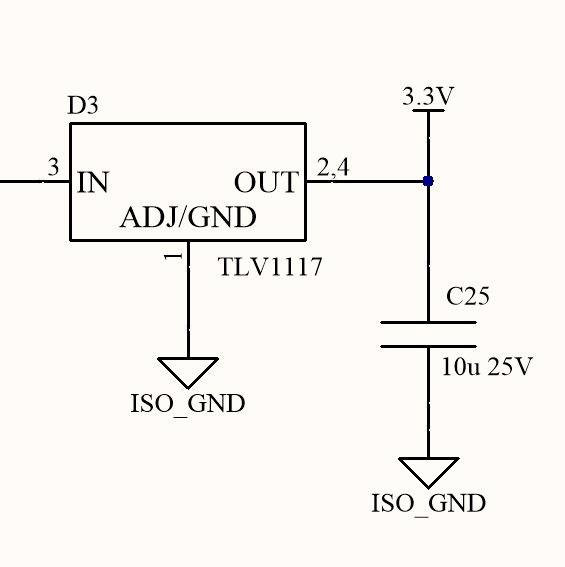
\includegraphics[scale = 0.6]{ris324.png}
    \caption{Схемотехническое решение на базе TLV1117}
    \label{ris:324}
\end{figure}

Отсутствие входной емкости обусловлено достаточным уровнем фильтрации сигнала на изолированном выходе 
DC-DC преобразователя, выходная емкость была выбрана значением 10 мкФ в соответствии с документацией 
на стабилизатор \cite{TLV1117:datasheet}. 

\subsection{Источник питания преобразователя уровней}
\hspace{1cm}

В качестве источника питания преобразователя уровней или отлаживаемых устройств (опционально) было решено 
использовать понижающий ШИМ-регулятор ST1S10, который способен обеспечить выходной ток до 3 А. 
Применяемая нами схема с его участием изображена 

на рисунке \ref{ris:ST1S10}

\begin{figure}[H]
    \centering
    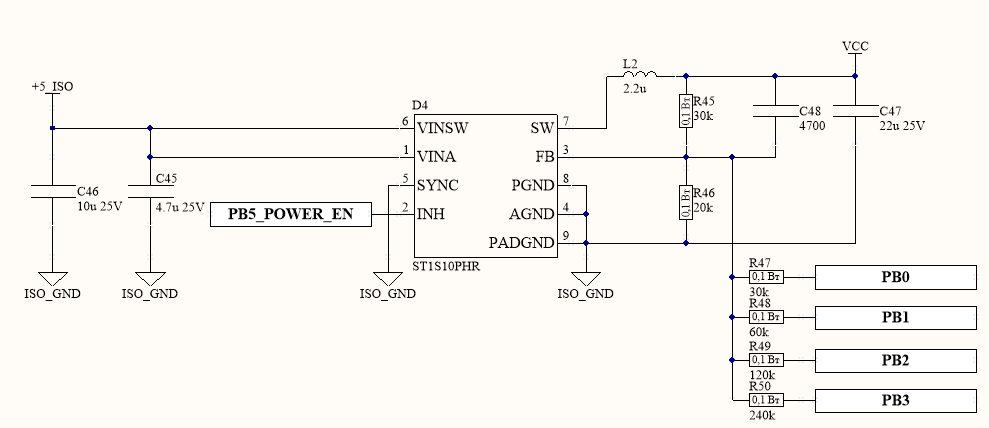
\includegraphics[scale = 0.7]{ST1S10 scheme.png}
    \caption{Схемотехническое решение на базе ST1S10}
    \label{ris:ST1S10}
\end{figure}

Здесь вывод VINSW предназначен для подачи входного напряжения питания, к нему подключается фильтрующий 
конденсатор C46. Вывод VINA -- для подачи входного аналогового напряжения, которому так же подключается 
фильтрующий конденсатор. 

Вывод INH являюется запрещающим, с активным низким уровнем, на него подается сигнал запрета работы от 
микроконтроллера. 

Если вывод SYNC подключен к земле, то регулятор работает на частоте 900 кГц, в иных случаях к этому выводу 
следует подключать внешний кварцевый генератор с тактовой частотой от 400 кГц до 1,2 МГц. В нашей схеме 
будем использовать частоту работы по умолчанию -- 900 кГц, подключив SYNC к земле. 

Выводы PGND, AGND, PADGND в нашей схеме подключаются к земле. 

С вывода SW снимается выходной ШИМ-сигнал, который подается на индуктивность L2, которая вместе с 
выходной емкостью C47 образуют LC-фильтр нижних частот, который выпрямляет ШИМ с SW. 

Для возможности подключения емкостной нагрузки значением более чем 100 мкФ необходимо добавить в схему 
конденсатор C48 с номиналом 4,7 нФ. 

Резисторы R45 -- R50 образуют делитель напряжения, средняя точка которого приходит на вывод FB, тем самым 
обеспечивая регулировку выходного с ST1S10 напряжения. 

Выходное напряжение рассчитывается по формуле \ref{eq:VoutST1S10}

\begin{equation}
    V_{out} = \frac{R45 \cdot 0,8}{R46 || r} + 0,8 
    \label{eq:VoutST1S10}
\end{equation}

, где r -- сопротивление некоторых из резисторов R47, R48, R49, R50, 
в зависимости от управляющих сигналов, поступивших с выводов микроконтроллера  PB0, PB1, PB2, PB3 
соответственно. Такая регулировка позволяет за счет отключения или подключения резисторов управлять 
выходным напряжением с ST1S10 в диапазоне от 2 В -- случай когда ни один из резисторов не подключен к 
выводу FB, до 3,5 В \cite{ST1S10:datasheet}. 


\section{Расчет элементов схемы}
\subsection{Исходные данные}
\hspace{1cm} 

Перед расчетом элементов обвязки DC-DC преобразователя следует определиться с исходными данными:

\begin{itemize}
    \item Диапазон входных напряжений от $U_{in.min.}$ = 12 В, что соответствует напряжению
    внешнего источника питания, до $U_{in.max}$ = 57 В, что соответсвтует максимальному
    напряжению с выхода контроллера PoE. 
    \item Частота ШИМ-контроллера, встроенного в LMR36520 равна $f_{sw}$ = 400 кГц 
    \cite{LMR36520:datasheet}. 
    \item Выходное напряжение на неизолированном выходе $U_{out1}$ = 5,5 В, максимальный 
    выходной ток этого выхода примем $I_{out1}$ = 50 мА для подключения светодиода и запаса 
    , который может понадобиться в ходе доработок и отладки устройства. 
    \item Выходное напряжение на изолированном выходе $U_{out2}$ = 5,5 В, но с возможностью допуска
    до 6,5 В из-за того, что это напряжение подается на преобразователь 3,3 В, который допускает 
    такое входное напряжение. Максимальный ток изолированного выхода примем равным $I_{out2}$ = 1 А,
    что обусловлено потребляемым током Wi-Fi решений и сотовых модемов в пике во время передачи 
    данных. 
    \item Падение на диоде VD7 примем равным $U_{f}$ = 0,5 В - типичное для выпрямительных диодов Шоттки, 
    в дальнейшем, при подборе диода, уточним его.
    
\end{itemize}

\subsection{Расчет индуктивности}
\hspace{1cm} 

Коэффициент трансформации $dN$ рассчитывается по формуле \ref{eq:dN}:

\begin{equation}
    dN = \frac{U_{out2} + U_{f}}{ U_{out1}} = \frac{5,5 + 1}{5,5} = 1,091
    \label{eq:dN}
\end{equation}

Из формулы \ref{eq:dN} видно, что если взять связанные индуктивности с коэффициентом 
трансформации равным 1, то это будет допустимой потерей точности расчетов. 

Далее введем минимальный коэффициент заполнения ШИМ $D_{min}$, который рассчитывается по 
формуле \ref{eq:Dmin}:

\begin{equation}
    D_{min} = \frac{U_{in.min}}{U_{in.max}} = \frac{12}{57} = 0,096
    \label{eq:Dmin}
\end{equation}

А максимальный коэффициент заполнения ШИМ равен $D_{max}$ = 0,5, что обуславливается внутренними
конструктивными ограничениями LMR36520. Коэффициенты заполнения показывают степень зарядки 
катушки индуктивности, чем больше $D$, тем больше успеет запастись энергии в катушке, для дальнейшей
передачи на выход схемы, и наоборот, чем меньше коэффициент заполнения, тем энергии будет меньше. 

Индуктивность катушки рассчитывается по формуле \ref{eq:L}:

\begin{equation}
    L =
    (U_{in. max} \cdot U_{out1}) \cdot \frac{D_{min}}{\Delta i \cdot f_{sw}} = 
    57 \cdot 5,5 \cdot \frac{0,096}{0,35 \cdot 400000} =
     3,549 \cdot 10^{-5}  \text{ Гн,}
    \label{eq:L}
\end{equation}

где $\Delta i$ отражает пиковую пульсацию тока намагничивания и устанавливается
в диапазоне от 30\% до 40\%. Было взято среднее значение в 35\%. 

Получившуюся по формуле \ref{eq:L} индуктивность L1 выберем ближайшей из доступного номинала 
индуктивностей серии MSD1278, компании CoilCraft \cite{MSD1278:datasheet}. Получилось, что L1 = 33 мкГн. 

Поскольку ток намагничивания совпадает с типичной формой тока дросселя, мы можем рассчитать пульсации 
тока от пика до пика $\varDelta i_{m}$, используя уравнение \ref{eq:dIm}

\begin{equation}
    \varDelta i_{m} =
    \frac{(U_{in.max} - U_{out1}) \cdot D_{min}}{L \cdot f_{sw}} =
    \frac{(57 - 5,5) \cdot 0,096}{33 \cdot 10^{-6} \cdot 400000} =
    0,376 \text{ А}
    \label{eq:dIm}
\end{equation}

Далее нужно оценить пиковые значения положительного и отрицательного токов выбросов при переключении
управляющего транзистора, который встроен в микросхему LMR36520. 

Пиковый положительный ток выброса $I_{pospk}$ рассчитывается по формуле \ref{eq:Ipospk}:

\begin{equation}
    I_{pospk} =
    I_{out1} + (dN \cdot I_{out2}) + \frac{\Delta i_{m}}{2} = 
    0,05 + (1 \cdot 1) + \frac{0,376}{2} =
    1,238
    \label{eq:Ipospk}
\end{equation}

Ограничение на положительный пиковый ток задается внутренним строенимем LMR36520 и равно 2,4 А, что больше
полученных нами 1,234 А при расчетах. 

Исходя из ограничения на отрицательный пиковый ток, равное -1,7 А, уравнение \ref{eq:Ioutmax} задает 
максимальный выходной ток изолированного выхода.

\begin{equation}
   I_{out2.max} = \frac{(1,7 - \frac{\Delta i_{m}}{2} + I_{out2}) \cdot (V_{in} - V_{out1})}{2 \cdot V_{out2}}
\label{eq:Ioutmax}
\end{equation}


При входном напряжении равным 12 В по формуле \ref{eq:Ioutmax} получается, что $I_{out2.max}$ = 0,923, 
что меньше заданного нами одного ампера. Однако, при входном напряжении равным 12,6 В 
$I_{out2.max}$ = 1,008 А, что уже нам подходит. \cite{LMR36520:Aplication Note}. 

\subsection{Расчет выходной емкости неизолированного выхода}
\hspace{1cm} 

Рекомендуемое значение емкости выходного конденсатор рассчитывается по формуле \ref{eq:Cout1}:

\begin{eqnarray}
    C_{out1} =
    \frac{\Delta I_{out1}}{f_{sw} \cdot \Delta U_{out1} \cdot K} \cdot 
    [(1 - D_{min}) \cdot (1 + K) + \frac{K^{2}}{12} \cdot (2 - D_{min})] = \nonumber\\
    \frac{0,05}{400000 \cdot 0,05 \cdot 0,4} \cdot 
    [(1 - 0,115) \cdot (1 + 0,4) + \frac{0,4^{2}}{12} \cdot (2 - 0,115)]  =\nonumber \\
    7,905 \cdot 10^{-6} \text{ Ф, }
    \label{eq:Cout1}
\end{eqnarray}

где $\Delta I_{out1}$ -- переходный выходной ток, равный 50 мА, $\Delta U_{out1}$ -- переходное выходное 
напряжение, равное 50 мВ,
K -- коэффициент пульсаций. 

Так же рассчитаем предельное максимальное эквивалентное последовательное сопротивление конденсатора (ESR),
 которое поможет 
нам при подборе типа выходного конденсатора, по формуле \ref{eq:ESR1}:

\begin{eqnarray}
    ESR = \frac{(2 + K) \cdot (\Delta U_{out1})}{2 \cdot \Delta I_{out1} \cdot 
    [1 + K + \frac{K^{2}}{12} \cdot (1 + \frac{1}{1 - D_{min}})]} = \nonumber\\
    \frac{(2 + 0,4) \cdot (0,05)}{2 \cdot 0,05 \cdot 
    [1 + 0,4 + \frac{0,4^{2}}{12} \cdot (1 + \frac{1}{1 - 0,115})]} =
    0,84 \text{ Ом}
    \label{eq:ESR1}
\end{eqnarray}

Теперь можно оценить значение выброса напряжения при пиковом токе по формуле \ref{eq:Vr1}:

\begin{equation}
    V_{r} = \Delta I_{out1} \cdot \sqrt{ESR^{2} + \frac{1}{(8 \cdot f_{sw} \cdot C_{out1})^{2}}} =
    0,05 \cdot \sqrt{0,99^{2} + \frac{1}{(8 \cdot 400000 \cdot 1,129 \cdot 10^{-4})^{2}}} =
    0,016 \text{ В}
    \label{eq:Vr1}
\end{equation}

При выходном напряжении 5,5 В значение выброса напряжения равно 0,016 В, что составляет всего лишь 0,3\%. 
\cite{LMR36520:Aplication Note}.

\subsection{Расчет выпрямительного диода}
\hspace{1cm} 

Рассчитаем обратное напряжение, то которое должен выдержать выпрямительный диод по формуле \ref{eq:VD} 
\cite{LMR36520:Aplication Note}:

\begin{equation}
    U_{d} = U_{out2} + dN \cdot (U_{in. max.} - U_{out1}) =
     5,5 + 1 \cdot (57 - 5,5) = 48 \text{ В}
    \label{eq:VD}
\end{equation}

Так же требованиям к диоду являются возможность пропускать через себя продолжительный ток в 1 А и частота
переключения в 400 кГц. По итогу можно взять диод Шоттки MBRS260T3G, который подходит под все требования 
\cite{MBRS260T3G:datasheet}.

\subsection{Выходная емкость изолированного выхода}
\hspace{1cm}

К выходу изолированного напряжения будут подключаться все основные компоненты, поэтому уровень пульсаций 
здесь более критичен, чем в неизолированном. 

Выходная емкость изолированной линии вычисляется по формуле \ref{eq:C2}:

\begin{equation}
    C_{out2} = \frac{I_{out2} \cdot D_{max}}{f_{sw} \cdot \Delta U_{out2}} =
    \frac{1 \cdot 0,5}{400000 \cdot 0,05} =
    2,5 \cdot 10^{-5} \text{ Ф}
    \label{eq:C2}
\end{equation}

, где $\Delta I_{out2}$ -- переходной выходной ток изолированного выхода, равный 1 А, а $\Delta U_{out2}$ --
переходное выходное напряжение на изолированном выходе, равное 50 мВ

ESR этого конденсатора рассчитаем по формуле \ref{eq:ESR1}.  Подставив вместо $\Delta I_{out1}$ 
в это уравнение $\Delta I_{out2}$, получим максимальное допустимое ESR равное 0,042 Ом.

Так же оценим пульсации по формуле \ref{eq:Vr1}, совершив те же замены, что мы делали для прошлой формулы. 
Получим значение напряжения пульсаций на изолированном выходе равным 51 мВ \cite{LMR36520:Aplication Note}. 


\subsection{Цепь обратной связи}
\hspace{1cm}

Резистор R19 верхнего плеча делителя обратной связи возьмем рекомендуемого номинала 100 кОм, тогда резистор
R20 нижнего плеча вычисляется по формуле \ref{eq:Rfb} \cite{LMR36520:datasheet}:

\begin{equation}
   R_{fbb} = \frac{R_{fbt}}{U_{out} - 1} =
   \frac{100000}{5,5 - 1} = 2,222 \cdot 10^{4} \text{ Ом}
    \label{eq:Rfb}
\end{equation}

Возьмем ближайший по ряду номиналов E24 -- 22 кОм. 


\subsection{Снабберная цепь}
\hspace{1cm}

Паразитная индуктивность утечки L1 $L_{leak}$ = 0,56 мкГн \cite{MSD1278:datasheet}. 

Паразитная емкость утечки диода VD7 $С_{leak}$ оценочно равна 28 пФ \cite{MBRS260T3G:datasheet}. 

Номинал резистора R18 снабберной цепочки рассчитывается по формуле \ref{eq:Rsnub}.

\begin{equation}
    R_{snub} = \frac{1}{2} \cdot \sqrt{\frac{L_{leak}}{C_{leak}}} = 
    \frac{1}{2} \cdot \sqrt{\frac{0,56 \cdot 10^{-6}}{28 \cdot 10^{-12}}} =
    70,711 \text{ Ом}
    \label{eq:Rsnub}
 \end{equation}

Номинал емкости конденсатора C20 снабберной цепи рассчитывается по формуле \ref{eq:Csnub}

\begin{equation}
    C_{snub} = \frac{1}{2 \cdot \pi \cdot R_{snub} \cdot f_{tank}} =
    \frac{1}{2 \cdot \pi \cdot 70,711 \cdot 40 \cdot 10^{6}} =
    5,27 \cdot 10^{-11} \text{ Ф}
    \label{eq:Csnub}
 \end{equation}

, где $f_{tank}$ -- частота подавляемого сигнала снабберной цепочкой, который экспериментально был установлен
равным примерно 40 МГц. 

В процессе работы снабберная цепь рассеивает на резисторе мощность подавляемого сигнала, из-за чего необходимо 
рассчитать эту рассеиваемую на резисторе мощность по формуле \ref{eq:Psnub} \cite{Snubber:calculation}. 

\begin{equation}
P_{snub} = C_{snub} \cdot U_{vd}^{2} \cdot f_{sw} =  
5,27 \cdot 10^{-11} \cdot 57^{2} \cdot 400000 =
0,0685 \text{ Вт}
\label{eq:Psnub}
\end{equation}

Полученная рассеиваемая мощность говорит нам о том, что smd-резистора типоразмера 0603 должно хватить, 
так как он способен рассеять на себе 0,1 Вт. 

\section{Результаты тестирования}
\hspace{1cm} 

Важным этапом разработки устройства является макетирование отдельных узлов. В этом разделе представлены 
результаты этапа макетирования подсистемы питания. В качестве измерительного оборудования использовался 
осциллограф компании Rigol марки DHO 1204 с 12-битным разрешением и полосой пропускания 200 МГц. Ограничение 
полосы выключено, импеданс щупа 1 МОм, делитель щупа 1:10. 

Начнем анализ схемы с проверки основных узлов DC-DC преобразователя. В качестве входного напряжения подадим
сигнал с лабораторного источника питания. Будем подавать на вход поочередно 12 В, 18 В, 24 В, 36 В и 48 В и 
отслеживать напряжение на выводе SW, падение напряжения на выпрямительном диоде и напряжение на изолированном
выходе схемы. 

Осциллограммы при входном напряжении 12 В представлены на рисунке \ref{ris:331}:

\begin{figure}[H]
    \centering
    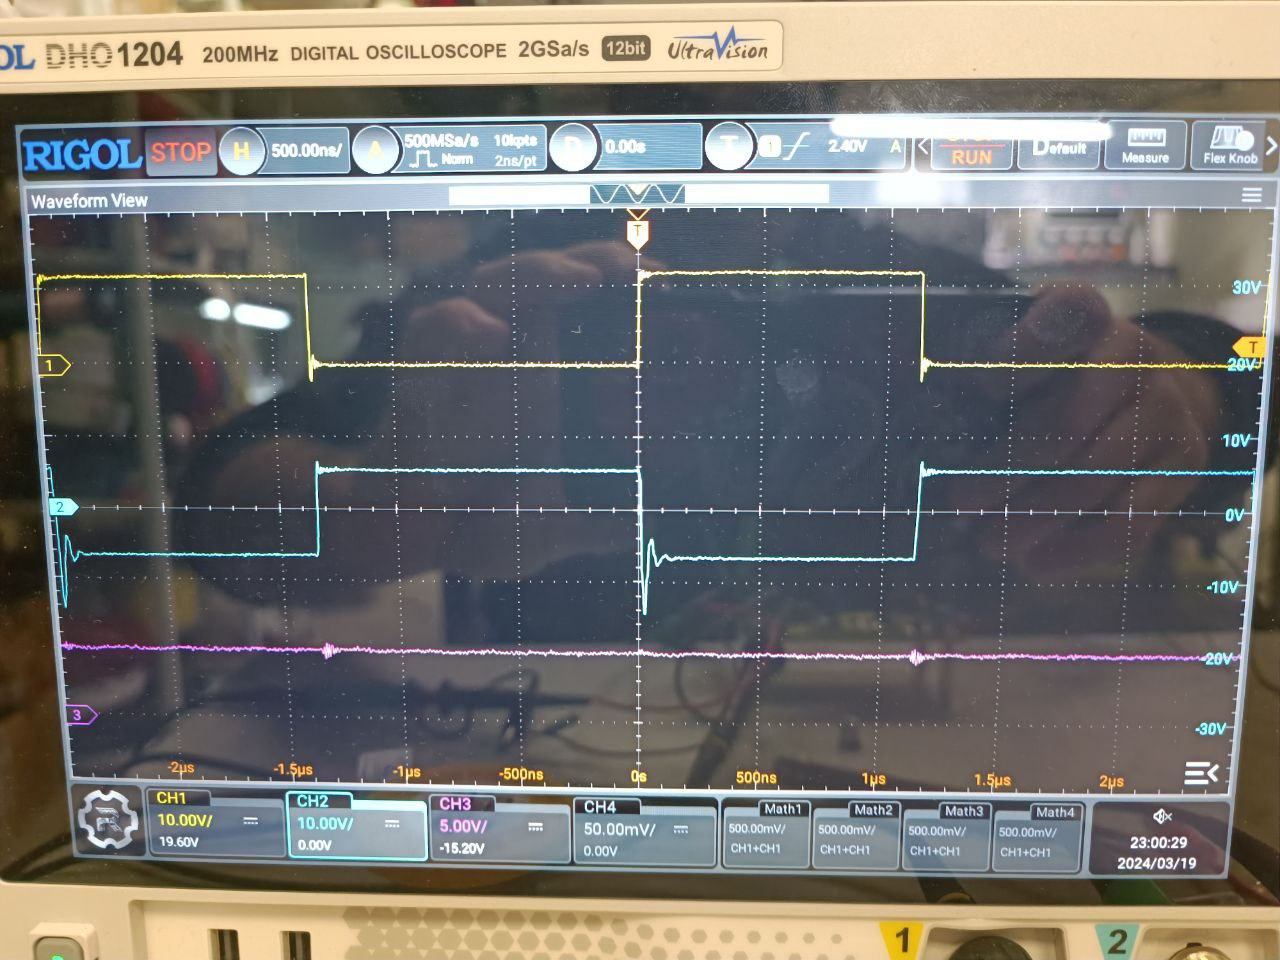
\includegraphics[scale = 0.4]{ris331.jpeg}
    \caption{Осциллограммы при входном напряжении 12 В}
    \label{ris:331}
\end{figure}

Здесь и далее желтый сигнал -- на выводе SW, развертка по напряжению 10 В/деление. Голубой сигнал -- падение 
напряжения на диоде (VD7, рисунка \ref{ris:321}), развертка по напряжению 10 В/деление. Фиолетовый сигнал -- 
контроль напряжения на изолированном выходе (контрольная точка CP5, рисунка \ref{ris:321}), развертка
по напряжению 5 В, нагрузка - 10 Ом. 

Осциллограммы при входном напряжении 18 В представлены на рисунке \ref{ris:332}:

\begin{figure}[H]
    \centering
    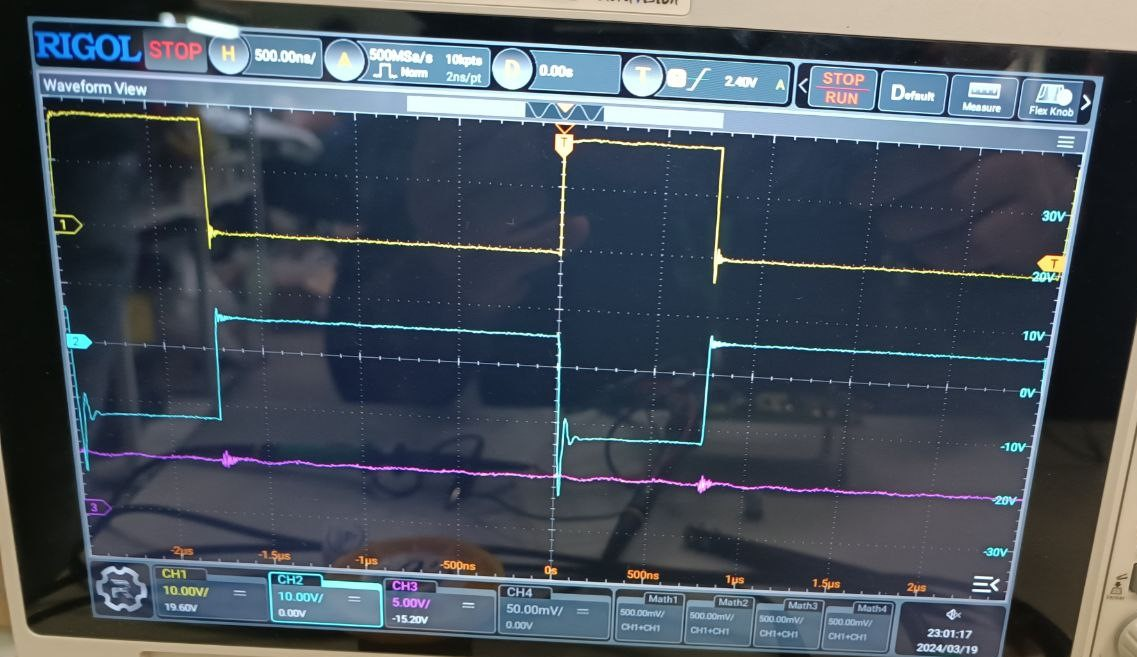
\includegraphics[scale = 0.6]{ris332.jpeg}
    \caption{Осциллограммы при входном напряжении 18 В}
    \label{ris:332}
\end{figure}

Осциллограммы при входном напряжении 24 В представлены на рисунке \ref{ris:333}:

\begin{figure}[H]
    \centering
    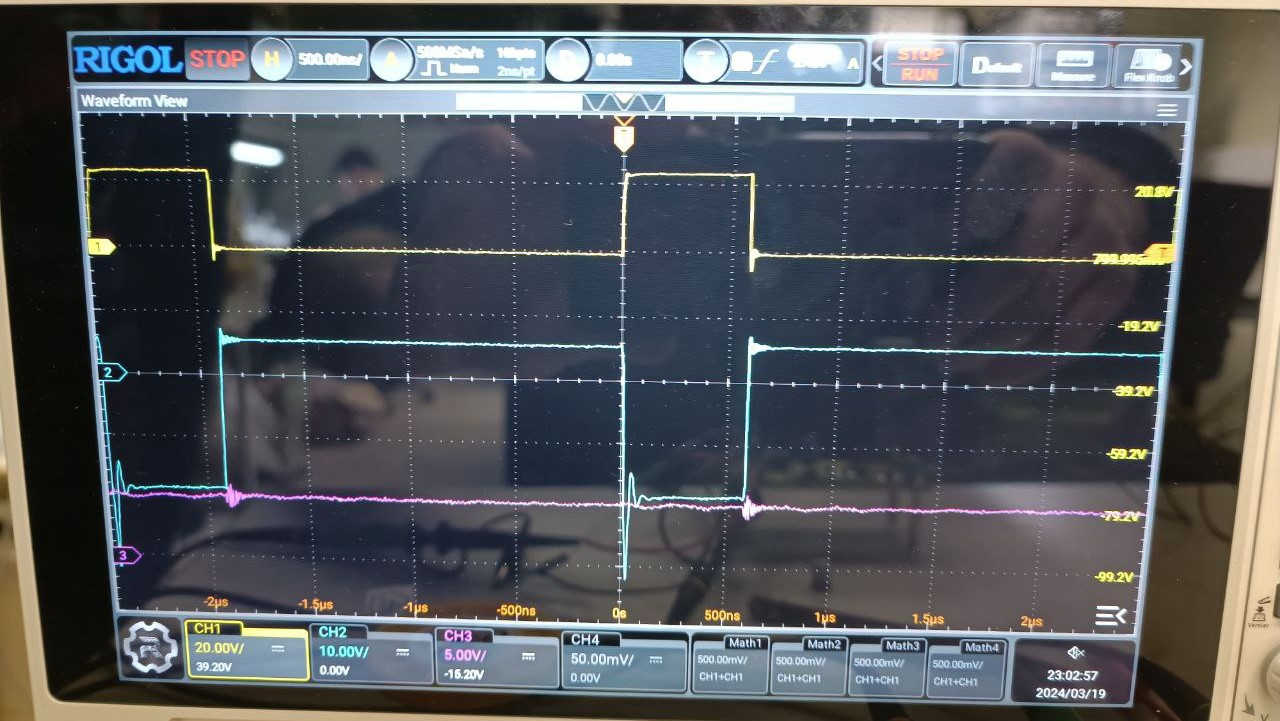
\includegraphics[scale = 0.5]{ris333.jpeg}
    \caption{Осциллограммы при входном напряжении 24 В}
    \label{ris:333}
\end{figure}

Здесь поменялась развертка желтого сигнала на 20 В/деление. 

Осциллограммы при входном напряжении 36 В представлены на рисунке \ref{ris:334}:

\begin{figure}[H]
    \centering
    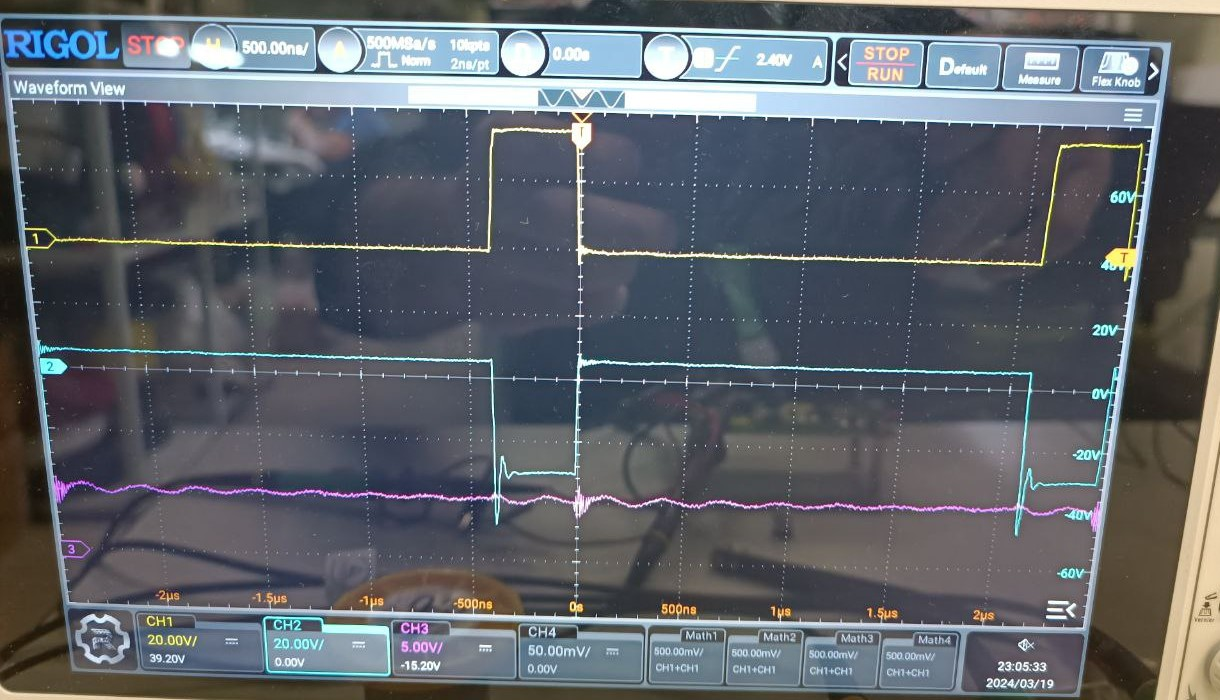
\includegraphics[scale = 0.55]{ris334.jpeg}
    \caption{Осциллограммы при входном напряжении 36 В}
    \label{ris:334}
\end{figure}

Здесь поменялась развертка голубого сигнала на 20 В/деление. 

Осциллограммы при входном напряжении 48 В представлены на рисунке \ref{ris:335}:

\begin{figure}[H]
    \centering
    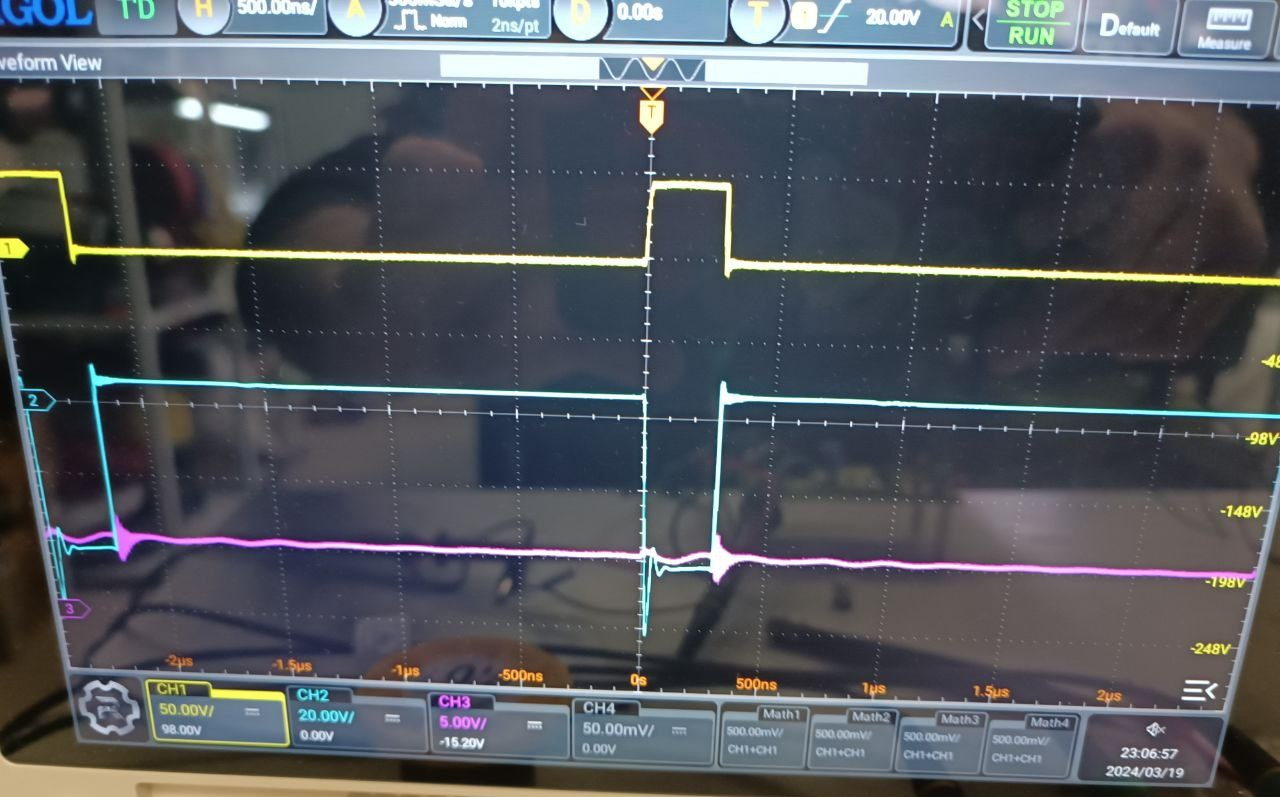
\includegraphics[scale = 0.5]{ris335.jpeg}
    \caption{Осциллограммы при входном напряжении 48 В}
    \label{ris:335}
\end{figure}

Здесь поменялась развертка желтого сигнала на 50 В/деление. Уменьшим развертку по времени до 100 нс/деление
и рассмотрим осциллограммы на рисунке \ref{ris:336}


\begin{figure}[H]
    \centering
    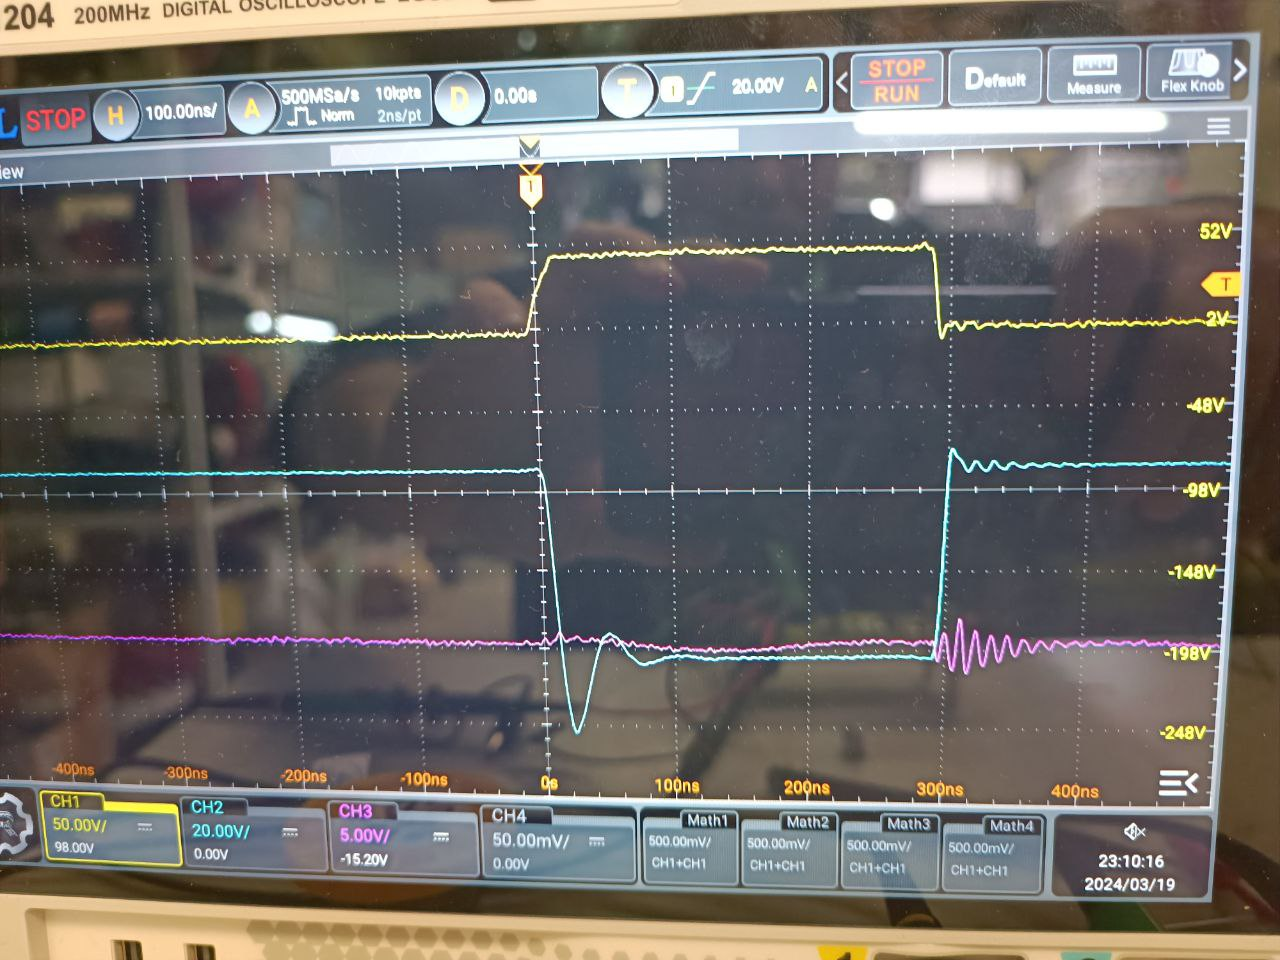
\includegraphics[scale = 0.4]{ris336.jpeg}
    \caption{Увеличенные осциллограммы при входном напряжении 48 В}
    \label{ris:336}
\end{figure}

На диоде (голубой сигнал), отчетливо видны выбросы индуктивности при переключении внутреннего транзистора. 
Амплитуда этих выбросов составляет -62 В при включении транзистора, и примерно 4 В при выключении.
Амплитуда отрицательных выбросов говорит нам о том, что следует заменить диод на тот, обратное напряжение которого
составляет хотя бы 100 В, а не 60, как сейчас. Основные искажения на изолированное питание вносят выбросы при 
выключении транзистора, амплитуда которых составляет примерно 1,5 В (размах 3 В), а частота 66,67 МГц. 
Расположенный дальше по схеме стабилизатор должен спокойно выдержать такие амплитуды выбросов, так же при
проектировании подсистемы питания мы закладывали возможность повышения выходного напряжения изолированного 
выхода до 6,5 В, что вписывается в расчетные данные. В случае неправильной работы LDO, можно будет попробовать
подавить высокочастотные выбросы добавлением входного конденсатора по входу стабилизатора 3,3 В.

Далее проанализируем работу PoE-преобразователя. Для понимания правильности его работы достаточно посмотреть
на осциллограмму на рисунке \ref{ris:337}:

\begin{figure}[H]
    \centering
    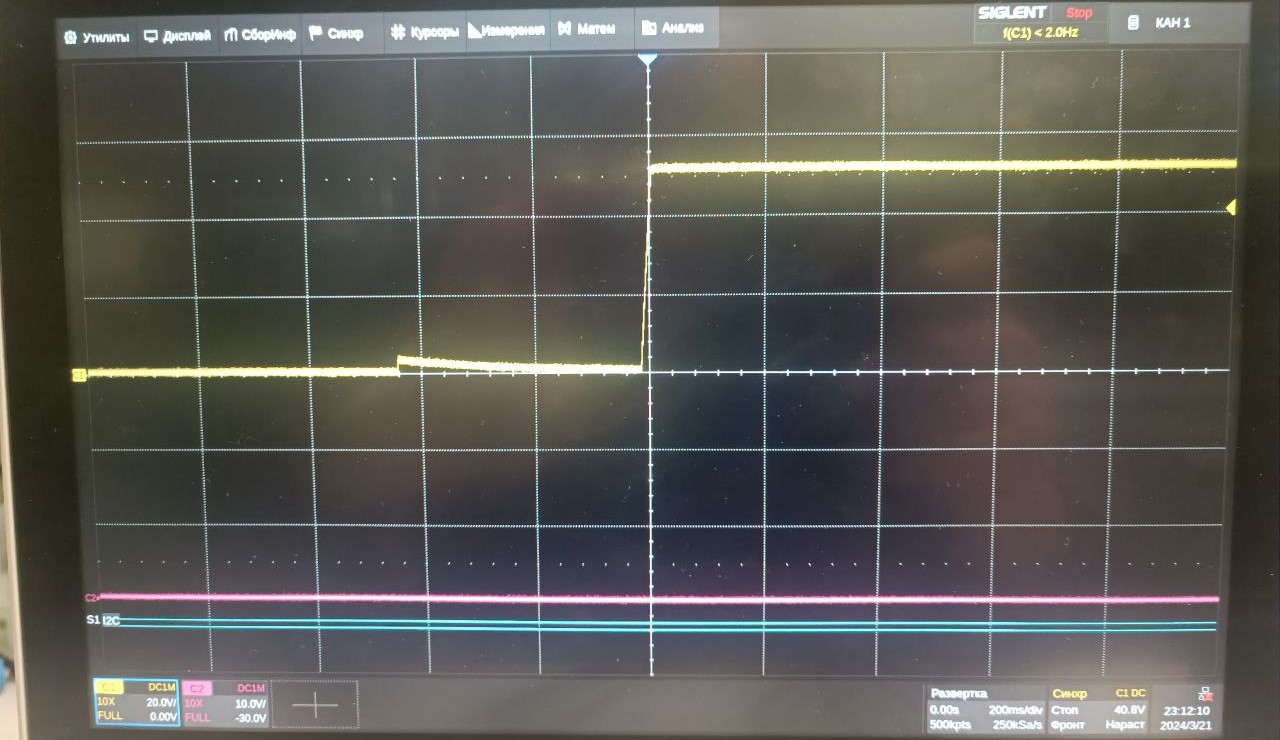
\includegraphics[scale = 0.45]{ris337.jpeg}
    \caption{Осцилограммы при старте работы PoE-контроллера}
    \label{ris:337}
\end{figure}

где, желтая осциллограмма -- вывод VDD, развертка по напряжению 20 В/деление, а по времени 200 мс/деление. 
В качестве нагрузки стоит LMR36520 нагруженный на 10 Ом.
Здесь можно заметить ярко выраженную стадию detection, которая длится 
примерно 100 мс, что соответствует документации на TPS2376. Этап классификации устройства проходит линейно и 
дальше контроллер выходит на напряжение питания равное примерно 60 В. 

За исключением выбросов на диоде VD7, схема работает как планировалось, расчеты соответствуют действительности.
